

\documentclass[12pt]{book}
%\usepackage[paperwidth=6in,paperheight=9in,margin=1.2in]{geometry}
\usepackage[a4paper]{geometry}

\usepackage{mystyle}
\usepackage{hyperref}
 
\title{TrainABA Supervision Curriculum Series\\ Volume 1: BCBA Reference Manual \\Second Edition}
\author{B. Theisen}
\date{April 21, 2019}
\makeindex[intoc]
 \renewcommand*{\marginfont}{\color{NavyBlue}\bfseries\sffamily}
\begin{document}
%include{path/to/title.tex}
     \maketitle
     \tableofcontents
     \listoffigures
     \listoftables
%% Uncomment sections to be included here. 
%% Note that sections cannot be nested. List everything here. Treat this text file as the sole index for calling which sections  to include in the book you are compiling.
% 

\documentclass[float=false, crop=false]{standalone}
\usepackage[subpreambles=true]{standalone}
\usepackage{import}
\begin{document}
\chapter{Administration}
This is a whole chapter about administration for supervisors. None of it is dependent on implementing procedures of certification or licensing entitities. For example, \underline{\texttt{\colorbox{Dandelion}{Fourier series}}}
\marginnote{Fourier Series}
\index{Fourier series}
gets indexed for no apparent reason.

Say, do you remember that image of space from last chapter? Here is the image, presented as a figure. Look how pretty a figure can be!
\begin{figure}[h]
    \centering
    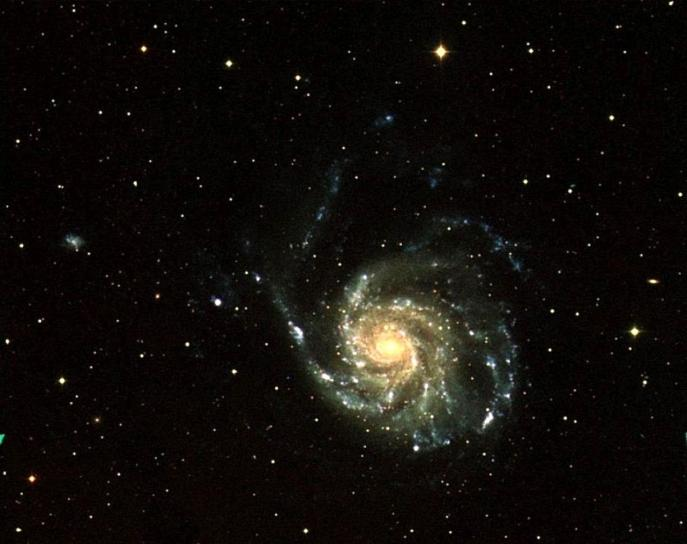
\includegraphics[width=0.25\textwidth]{space}
    \caption{A nice space.}
    \label{fig:space1}
\end{figure}
 
As you can see in the figure \ref{fig:space1}, the 
function grows near 0. Also, in the page \pageref{fig:space1} 
is the same example.
 
All of this continues to another page, which includes a bulleted list.
\begin{itemize}
\item fun
\item sun 
\item rock
\item roll
\item magic
\item fun
\item space
\item more
\item okay
\end{itemize}


The most important consideration is the use of power when microwaving burritos. Whether at a concert or anywhere that sells gasoline, burritos and microwaves are your friends. These are the friends you want to keep. Parents encourage their kids to have these lasting relationships. 

A \textcolor{orange}{TikZ}
\marginnote{TiKZ} 
\index{TikZ}
 figure will be rendered below this line. It has to get to the next page first. Be sure to hold your excitement for the moment. It really will be ready to show momentarily. Any old moment. Could be this one. Maybe now? 
 \begin{figure}[ht]
 \subimport{../}{diagram.tex}
 \label{fig:tikzexample}
\caption{A nice simple diagram}
\end{figure}
 ...
\end{document}



 \documentclass[float=false, crop=false]{standalone}
\usepackage[subpreambles=true]{standalone}
\usepackage{import}
\usepackage{hyperref}
\begin{document}
\chapter{About This Book}

A typical book is mostly written by the author whose name is on the cover. The book is completed by staff members at a publishing company. The person in charge of typesetting is usually not an expert on the subject the book presents, which can lead to typesetting decisions that confuses readers. An ebook is available if the publisher can secure digital rights management (DRM) procedures to prevent the book from being shared. The materials are copyrighted such that only the publisher can give permission for its content to be printed elsewhere. It is sold and distributed for a profit. The author is paid a royalty.

This is not a typical book. It was written by the author whose name is on the cover, though it was openly workshopped using a version control system allowing anyone to give input. The book was completed by a staff of one at a nonprofit. Mostly, their job was to program free and open source software to handle the publishing process automatically. The typesetting was programmed by the author, leading to typesetting decisions that were congruent with the contents. An ebook was compiled using the same code base as the paper copy. It was made freely available to others, along with the source code, without DRM, to promote sharing.

The materials were copyrighted using a Creative Commons 4.0 - Attribution - Sharealike - Non-commercial license, to provide readers with the freedom to use, copy, modify, and distribute the book non-commercially. These modified or copied versions retain the same freedoms as the original work. There is no need to ask the publisher for permission to reprint the book's contents. The book is distributed freely with paper copies sold at a reasonable price. The profits go to a public charity that advances the contents of the book. The author is not paid a royalty.

\section{History of the TrainABA Supervision Curriculum Series}
This book originated from a project fromTrainABA, a startup organization from 2013-2016. Its goal was to function as a publisher and resource for behavior analysis supervision. It was unsuccessful. When TrainABA closed, the publisher released its works under a Creative Commons 4.0 - Attribution - Sharealike - Non-commercial license. Some of its works survived as a project, such as the free Moodle Course, manuscripts, and SAFMEDs app. These works were donated to Cumulative Records Documentation Society, to be developed and archived for public use. 

\section{Publisher}
This book was published by Cumulative Records Documentation Society (CRDS), a 501(c)3 nonprofit based in Los Angeles, California, USA. CRDS produces archive-quality continuing education materials for public use. CRDS employs technical producers and project maintainers to develop and distribute works such as this. CRDS survives on the generosity of its members. To make a donation, or to become a member, please visit \url{http://cumulativerecords.org}.

\section{Author}
This book was written by Benjamin Theisen. He has a PhD in Business Psychology and MBA, both of which he earned while working full-time in Los Angeles, California. He is a Board Certified Behavior Analyst (\#1-10-7323) specializing in organizational behavior management. Dr. Theisen is an adjunct professor in the Industrial-Organizational/Business Psychology Department at The Chicago School of Professional Psychology's Los Angeles Campus. Dr. Theisen is a consultant at Defensible Personnel Systems, Inc. and contributes 30 hours per week of time to CRDS. He researches personnel in the applied behavior analysis profession. His hobbies include dance, music, mathematics, computers, and exercise.

\section{Collaboration Tools}
CRDS built this book using collaboration tools from software developers. Anyone can contribute or suggest changes for free. There will be a permanent public record of any such collaboration. We encourage readers to report errors using the Issue Tracker on our GitHub repository. The location is: \url{https://github.com/cumulativerecords/TrainABA-Vol1-BCBAReferenceManual/issues}

\subsection{Creating New Materials from This Book}
Readers may notice opportunities to use/extend the book's contents (e.g., build a slideshow to be used where one works or teaches). All readers are invited to suggest changes to this book using the GitHub repository. For readers who have modified the contents to be used where they work or teach, we ask that you submit your materials to CRDS so that we can make them available to other readers. We believe this will afford us the opportunity to have one or two well-developed versions of a work, which are compatible with the original book. We believe one organized version is better than multiple partially-developed, incompatible but similar works. 

Readers who create materials retain credit for their contributions. In many cases, CRDS will supply content creators with a technical producer who will help them organize the materials for larger audiences at no charge. Organizations who use CRDS materials regularly for personnel development provide donations.

\subsection{Online Documentation}
The materials in this book will likely be distributed as online documentation from \url{https://ReadTheDocs.org}. More information about this project will be made available at a later release. 

\section{Versions}
The typesetting system used to compile this work is very flexible. It can compile a similar version for nearly any page size with a very simple change in code. It is designed to provide maximum flexibility to readers, who are often supervisors and educators with a need to use only certain sections of this work. By downloading the source code, readers are able to pick and choose which sections of the book to compile. They can rebrand the book to indicate that they modified the original version. We encourage readers to tinker with the source code to download modified versions of the work. It is surprisingly easy to make a mobile-friendly version of this book. One can also make a new version for each month in a supervision setting, for example. It is very flexible. CRDS will provide a version sized for standard typing paper (A4 or 8 1/2" X 11") as well as a small version designed for mobile phones. To request a custom size or version, contact us through our website at \url{http://cumulativerecords.org/contact}.

\end{document}



% \include{sections/segment1/segment1}
     \printindex
\end{document}

